\chapter{Markov Decision Processes}
\label{ch_mdp}

TODO: Motivation.

We start by introducing Markov chains, a simpler type of probabilistic
processes which does not have non-determinism,
then continue to generalize to Markov Decision Processes.
We then overview known approaches to {\em verification} (checking if a
given MDP satisfies a given property) with special focus on Bounded
Real-Time Dynamic Programming which will be used in later chapters.

\section{Markov Chains}

Markov chain is a simpler formalism than
Markov decision process and provides a good first intuition about
probabilistic models. In a Markov chain there are no decisions, only
probabilities of transition.

\begin{definition}
    Markov chain.
\end{definition}

\begin{example}
    Let $s_0$ be the starting node (TODO: compute some
    probabilities).

\hfill \break
\centering
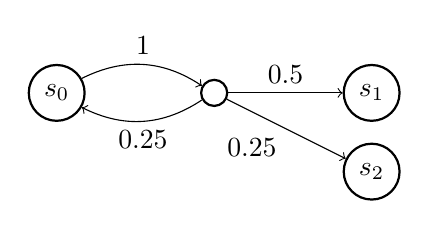
\begin{tikzpicture}
    \tikzstyle{state}=[thick,draw=black,circle]
    \tikzstyle{decision}=[draw,shape=circle,fill=black]

    \node[state] at (0,0) (s0) {$s_0$};
    \node[state] at (2,0) (s0b) {};
    \node[state] at (4,0) (s1) {$s_1$};
    \node[state] at (4,-1) (s2) {$s_2$};

    \draw (s0) edge [bend left, ->] node [midway, above] {$1$} (s0b);
    \draw[->] (s0b) -- (s1) node [midway, above] {0.5};
    \draw (s0b) edge [bend left, ->] node [midway, below] {0.25} (s0);
    \draw[->] (s0b) -- (s2) node [midway, below left] {0.25};
\end{tikzpicture}
\end{example}

TODO: Recommend some interesting markov chain literature.

\section{Markov Decision Processes}

Suppose a system similar to Markov chains.
If there are points when an actor interacting with the system can make
choices which affect the behaviour of the system it is called a Markov
Decision Process.

\begin{definition}
A {\em Markov Decision Process} is a tuple $(S, A, E, \Delta)$, where
$S$ is a finite set of states,
%$s \in S$ is the initial state,
$A$ is a finite set of actions,
$E : S \to \powerset{A}$ gives the set of enabled actions in a state,
and $\Delta : S \times A \to \distribution{S}$ is a partial transition
function which assigns a probability distrubution on states to an action
and a state.

It is assumed without loss of generality that for all $s \neq s'$ it
holds that $E(s) \cap E(s') = \emptyset$. If this didn't hold the
actions could be just renamed.
\end{definition}

\begin{example} The MDP $(\{s_0, s_1, s_2\}, \{a\}, E, \Delta)$,
    where
    $E(s_0) = \{a,b\}$, $E(s_1) = E(s_2) = \emptyset$,
    and $\Delta(s_0, a) = \{(s_1, 1)\}$,
    $\Delta(s_0, b) = \{(s_1, 0.5),$ $(s_2,0.25), (s_0,0.25)\}$
    is depicted below.

    The smaller black dots mark points of random transition. If an
    action leads to a state with probability one the random transition
    dot is omitted in the picture.

    The actor making decisions should choose action $a$ if
    they want to get to $s_1$, or (possibly repeatedly) choose $b$ if
    they want to get to $s_2$ (the achievement of this goal is not
    guaranteed).

\hfill \break
\centering
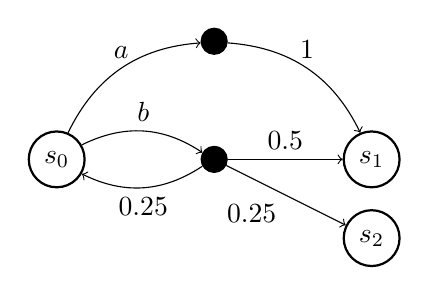
\begin{tikzpicture}
    \tikzstyle{state}=[thick,draw=black,circle]
    \tikzstyle{transition}=[draw,shape=circle,fill=black]

    \node[state] at (0,0) (s0) {$s_0$};
    \node[transition] at (2,1.5) (s0a) {};
    \node[transition] at (2,0) (s0b) {};
    \node[state] at (4,0) (s1) {$s_1$};
    \node[state] at (4,-1) (s2) {$s_2$};

    \draw (s0) edge [bend left, ->] node [midway, above] {$a$} (s0a);
    \draw (s0a) edge [bend left, ->] node [midway, above] {$1$} (s1);
    \draw (s0) edge [bend left, ->] node [midway, above] {$b$} (s0b);
    \draw[->] (s0b) -- (s1) node [midway, above] {0.5};
    \draw (s0b) edge [bend left, ->] node [midway, below] {0.25} (s0);
    \draw[->] (s0b) -- (s2) node [midway, below left] {0.25};
\end{tikzpicture}

\end{example}

\begin{definition}[Path]
    An {\em infinite path} is
    a sequence $\omega = s_0 a_0 s_1 a_1
    \ldots$ such that $a_i \in E(s_i)$ for all $i \in \mathbb{N}$.
    The set of all infinite paths of is denoted $IPaths$.

    A {\em finite path} is a prefix of an infinite path such that it
    ends with a state. The last state for a finite path $\rho$ is
    denoted $\last(\rho)$. The set of all finite paths is denoted
    $FPaths$.
\end{definition}

The following definition introduces what is commonly called strategy,
policy, scheduler or adversary. It is the decision maker in the MDP which
looks at the path traversed so far and assigns each action $a$
in the last (current) state the probability of $a$ being chosen.


\begin{definition}[Strategy]
    Let $\mathcal{M} = (S,A,E,\Delta)$ be a Markov decision process.
    A {\em strategy} is a function
    $\sigma : FPath \to Dist(A)$
    such that
    $\sigma(\rho)(a) > 0 \implies a \in E(\last(\rho))$.
\end{definition}

The technical condition at the end ensures that only actions which can
be chosen have non-zero probability assigned by the strategy.

What happens once the strategy is fixed? The MDP becomes a Markov chain.
This can be seen in the examples, e.g. if the strategy is to always
choose $b$, the MDP from Example 2 becomes the MC from Example 1.

For very small MDPs this gives the first algorithm for evaluating their
properties: for every strategy reduce the MDP to a Markov chain and evaluate the
property using known Markov chain algorithms, then aggregate the
results.

The idea of this naive method can be significantly improved and instead
of exploring a vast amount of strategies only a small portion of
reasonably good strategies is explored \parencite{smc} but that
technique is beyond the scope of this thesis.

TODO: Mention or prove that there exists an optimal memory free strategy
(this is in Puterman for reward maximization, does it hold for


Now we proceed to define {\em end components} -- parts of MDP which
allow for an infinitely repeated cycle of states and actions in a path.
These are of particular interest when sampling an MDP (as the sampling
agent might run in the MDP indefinitely).

\begin{definition}[End component]
Let $\mathcal{M} = (S, A, E, \Delta)$ be an MDP. An {\em end component}
is a pair $()$


Maximum end component.
\end{definition}

\noindent {\bf Observability of MDP.}
One can distinguish between various levels of knowledge about an MDP,
usually depending on the source of the model.
In partially observable MDPs the information about $\Delta$ may not be
available (but algorithms for solving the reachability
problem in such MDPs exist too \parencite{atva14}). In this thesis only
fully observable MDPs are studied.


\section{Verification}

{\em Formal verification} is the act of verifying that a given system satisfies
a given property. The result of a verification is a proof. {\em Model
checking} is an approach to formal verification which uses a model of
the system verify the property.

In our case the systems are modelled as Markov decision processes and
the properties are maximum probabilities of reaching a state.

\noindent \textbf{Reachability probability.}
$P^\sigma_{\mathcal{M},s}(\lozenge F)$

TODO: Whcih method give guarantees and which do not?

A description of the most common approaches to computing Pr... follows.
Value Iteration, Strategy Iteration and Interval Iteration are
standard algorithms which have to perform their computation on the
whole MDP resulting in significant computation time and memory
requirements. Further we describe BRTDP which is a heuristic with a
significant advantage on suitable models.

Another approach is formulating the problem as a system linear equations
and solving it. The solution is precise and has guaranteed correctness
but the computation quickly becomes expensive as the model grows in
size. We do not elaborate on this method -- the reader is referred to
\parencite{forejt}.

\subsection*{Computing Zero States}

Before introducing the algorithms we first need to calculate the set $Z$
of {\em zero states} for given MDP $\mathcal{M}$. These are states $z
\in Z$ such that for any $\sigma \in \Sigma$ it holds that
$P^\sigma_{\mathcal{M},z}(\lozenge F) = 0$. TODO.

\subsection{Value Iteration}

Value iteration (in its variation for computing maximum rewards) is a
dynamic programming algorithm which was first described by Richard
Bellman (known for introducing the term dynamic programming) in 1957
\parencite{bellman}.

The main idea is materialized in the following recurrence relation for
newly introduced variables $x_s^n, s \in S, n \in \mathbb{N}$.
\[
x_s^n =
\begin{cases}
    1 & \text{if }s \in F \\
    0 & \text{if }s \in Z \\

    \max_{a \in E(s)} \sum_{s' \in S} \Delta(s,a)(s') \cdot x_{s'}^{n-1}
    & \text{if }s \in S \setminus (F \cup Z)
\end{cases}
\]

TODO: Fix the relation.
By computing $x^n$ for $n = 1,2,\ldots$ we gain increasingly precise
estimate of the actual maximum reachability probability,
formally $\lim_{n \to \infty} x^n_s = P_{\mathcal{M},s}(\lozenge F)$.
TODO: prove!

This recurrence relation is now turned into a dynamic programming
algorithm as shown in \autoref{vi}. Instead of iterating $n$ times the
algorithm proceeds with its computations while the convergence is not
slow (the threshold is given by some $\epsilon$). Limit on the number of
iterations may be introduced if we want to check time bounded
properties.

\begin{algorithm}
\caption{Value Iteration}
\label{vi}
\begin{algorithmic}
    \State $\forall s \in S,\; s \gets$ if $x \in F$ then $1$ else $0$
    \Do
        \ForEach{$s \in S \setminus (F \cup Z)$}
            \State $x_s \coloneqq
                \max_{a \in E(s)} \sum_{s' \in S} \Delta(s,a)(s') \cdot x_{s'}$
        \EndFor
    \doWhile{the change of $x_s$ for any $s$ is greater than $\epsilon$}
\end{algorithmic}
\end{algorithm}

Value iteration is an easy method for computing the reachability
probability of a given MDP. It is doing extra work on models where only
a small part needs to be explored to find a good strategy as it has to
compute its results for all the states.

\subsection{Strategy Iteration}
Strategy Iteration (also Policy Iteration).
Describe origin
How it works
Pros and cons

\subsection{Interval Iteration}
Interval Iteration.
Describe origin and motivation.
How it works
Pros and cons

http://www.sciencedirect.com/science/article/pii/S0304397516307095
http://pageperso.lif.univ-mrs.fr/~benjamin.monmege/talks/MoVe2015.pdf

\section{Bounded Real-Time Dynamic Programming}

When only a portion of an MDP needs to be searched to find the right
strategy there is an opportunity to employ algorithms which avoid
searching the whole state space. Bounded Real-Time Dynamic Programming
(BRTDP) is such an algorithm. Originally developed for
the objective of finding the best-profit strategy
\parencite{profit_brtdp} the algorithm was adapted to the problem of
verification \parencite{atva14}.

Let us define the {\em value function} $V : S \times A \to
[0,1]$ for all $s \in S, a \in E(s)$ as follows

\[
    V(s,a) \coloneqq \sum_{s' \in S} \Delta(s,a)(s')V(s')
\]
(TODO: Define $\mathcal{M}$ which is used further)
BRTDP is learning $V$ by computing its lower and upper bounds $L, U$
through simulated runs of $\mathcal{M}$ from the given initial state.
TODO: CONTINUE explanation

Unfortunately this algorithm is not guaranteed to converge when the MDP
contains non-trivial end components. TODO: Picture with explanation

\begin{example}
\hfill \break
\centering
\begin{tikzpicture}
    \tikzstyle{state}=[thick,draw=black,circle]
    \tikzstyle{transition}=[draw,shape=circle,fill=black]

    \draw[<-] (s0) -- node[above] {} ++(-1cm,0);

    \node[state] at (0,0) (s0) {$s_0$};
    \node[state] at (2,0) (s1) {$s_1$};
    \node[transition] at (4,0) (s0b) {};
    \node[state] at (6,-0.7) (s2) {$s_2$};
    \node[state] at (6, 0.7) (s3) {$s_3$};

    \draw (s0) edge [bend left, ->] node [midway, above] {$a$} (s1);
    \draw (s1) edge [bend left, ->] node [midway, below] {$b$} (s0);
    \draw (s1) edge [->] node [midway, above] {$c$} (s0b);

    \draw[->] (s0b) -- (s2) node [midway, below] {0.5};
    \draw[->] (s0b) -- (s3) node [midway, above] {0.5};
\end{tikzpicture}
\end{example}

TODO: Explain how the algorithms gets modified to handle end components.

Prove PAC?


\begin{algorithm}
\caption{BRTDP for MDPs without end components}
\label{brtdp}
\begin{algorithmic}
\State $U(s,a) \gets 1, L(s,a) \gets 1 \; \forall s \in S, a \in E(s)$
\State $U(z,a) \gets 0, L(t,a') \gets 1
    \; \forall z \in zero states, a \in E(z)
    \; \forall t \in target states, a' \in E(t)$
\State $s \gets s_0$
\While{max diff in initial is greater than epsilon}
    % explore
    \State \# Explore Phase
    \While{$s \not \in target \cup zero$}
        \State $a \gets$ sample uniformly from
        \State $s \gets $ sample according
        \State $\omega \gets \omega \; a \; s$
    \EndWhile

    % update
    \State \# Update Phase
    \While{$s \neq s_0$}
        \State $pop(\omega)$
        \State $a \gets pop(\omega)$
        \State $s \gets last(\omega)$
        \State $U(s,a) \coloneqq \sum_{s' \in S} \Delta(s,a)(s')U(s')$
        \State $L(s,a)\, \coloneqq \sum_{s' \in S} \Delta(s,a)(s')L(s')$
    \EndWhile
\EndWhile
\State \Return Action from $v_0$ to the best node (by some
given metric).
\end{algorithmic}
\end{algorithm}
